\section{Problem 3: Design for Decision Model}
In this question, we play the role of management department. There are two parallel lanes in the “car zone” of the airport. We are required to set up a reasonable “boarding point”. Also, we need to arrange taxis and passengers and ensure the safety of vehicles and passengers. Under the conditions, the total ride efficiency is the highest. 
When there is no dispatch, it is easy for passengers to give priority to the vehicle on the side closer to themselves. There is no load on the side, or when driving to the opposite side of the road, the taxi in the passing lane causes a safety hazard. If you do not stipulate that you can only get on the train again, it will also cause the passengers behind you to choose the taxi behind, which is inefficient and dangerous. In addition, if the car is released too much, it will also lead to confusion. 
To summarize the above issues, we need to make provisions to facilitate scheduling.
\subsection{Assumptions}
\begin{sloppypar}
When a new flight arrives at the airport, passengers who need a taxi are required to register with the management department, and the management department also assigns the pick-up point that each passenger should go to. The taxi waits in the storage pool. According to the physical location of the relative storage pool at each loading point and the number of existing passengers, the management department allocates the loading point to the taxi in the storage pool, and the storage pool reaches the nearest one. The time of the vehicle is not counted. Since the many-to-many model has better efficiency, we also plan to use the multiple-to-multiple model.Therefore, for each boarding point, you can specify $k$ consecutive vehicles in the storage pool at a time. The car goes to the 
same pick-up point, and the first k passengers in the team can carry the 
baggage at the same time to get on the bus. Considering the efficiency and passenger safety, the upper vehicle point is set on the outside of the two parallel 
lanes, and only the overpass can be reached to the opposite vehicle, which
takes $t_{t}$ seconds.
The initial entrance position of the “carriage zone” is on one side of the
road, that is, the initial position of all passengers is on the same side,
named L side, the other side of the road is named R side, and the number 
of passengers on each boarding point on the same side As balanced as 
possible.
\end{sloppypar}
\subsection{Model establishment}
In terms of the setting of the boarding point, we have n loading points on the L side, and are lined up at the entrance of the “riding area”. The distance from the first boarding point to the boarding area is not counted. m pick-up points, and at the exit of the flyover, line up, the distance from the first pick-up point to the exit of the bridge is not counted. Set the distance between the vehicles to be $(d+k*\Delta d)$m. Considering the passenger's walking speed, it is necessary to $(d+k*\Delta d)$s to reach the next boarding point. After the passenger waits for the taxi, it takes c seconds to carry the luggage, and the taxi can enter the driving state.
Due to the topic, the total ride efficiency is the highest.
Among them, the passenger's total riding efficiency $E$:
\begin{equation} E = \frac{P}{T_s}\end{equation}

$P$ is the total number of passengers in a round of flights, and $T_{S}$ is the sum of the time when P passengers are waiting to board.
It can be seen that if E is as large as possible, the TS should be as small as possible, that is, all passengers should wait the least.
The time TS in which the passenger waits is composed of two parts: the total time $T_{a}$ taken by all the passengers to the boarding point, and the total time $T_{w}$ of all the passengers waiting at the boarding point to the current taxi. which is
\begin{equation} T_{s} = T_a+T_w\end{equation}
considering
\begin{equation} T_{a} = T_{aL}+T_{aR}\end{equation}
It is divided into two parts: the total time $T_{aL}$ used by the $L$ side passengers to get to the boarding point and the total time $T_{aR}$ used by the $R$ side passengers to get to the boarding point. Let the number of passengers on the $L$ side be $x$, and the number of passengers on the R side be $P-x$.

Considering $T_{aL}$, the time required for the passenger to go to the nearest first pick-up point is 0, and the second required time to go to the nearest $(d+k*\Delta d)*s$,..., to the nearest i The boarding time is $(d+k*\Delta d)*(i-1)$. $i$ is a natural number. The above assumes that the number of passengers at each boarding point is average, so the number of passengers at each boarding point on the L side is $\frac{x}{n}$.
Use the Gaussian summation formula, where n is the base
\begin{equation} T_{aL} = \frac{{(d+k*\Delta d)}*{(n-1)}*{x}}{2}\end{equation}
Consider $T_{aR}$ again, compared to $T_{aL}$, plus the passengers crossing the bridge $T_s$
\begin{equation} T_{aR} = \frac{{(d+k*\Delta d)}*{(m-1)}*{(p-x)}}{2}+t_t*(P-x)\end{equation}
Consider $T_w$, that is, the sum of the time that all passengers can wait until the current taxi can drive at the boarding point, which is the time $t_wf$ of each passenger waiting at the boarding point to wait for the current taxi to drive.
$T_wf$ also has two parts: each passenger needs to wait for the taxi to come time $t_1$ and each passenger needs to carry luggage, sit in the seat, wait for the taxi to enter the driving state time $t_2$
Consider $t_1$ first. According to the previous assumption, the taxi waits in the storage pool. According to the physical location of the relative storage pool and the number of existing passengers at each loading point, the management department allocates the waiting point to the waiting taxi. The time from the car pool to the nearest boarding point is not counted. Each time a batch of cars is issued, the quantity is $k(m+n)$, k is assigned to the same boarding point, k cars, m+n is all the boarding points. On average, each vehicle needs to drive all the entry points at a speed of $vm/s$, and because the number of points on the $L$ side and the $R$ side is different, they are:
\begin{equation} t_{1L} = \frac{{(d+k*\Delta d)}*{(n-1)}}{v*k}\end{equation}
\begin{equation} t_{1R} = \frac{{(d+k*\Delta d)}*{(n-1)}}{v*k}\end{equation}
After the Gaussian summation of the number of people
\begin{equation} T_{1L} = \frac{{(d+k*\Delta d)}*{(n-1)}*x}{v*k}\end{equation}
\begin{equation} T_{1R} = \frac{{(d+k*\Delta d)}*{(n-1)}*(p-x)}{v*k}\end{equation}
Considering $t_2$, each passenger needs to wait for all the passengers in front of him to carry the luggage into the car. Each person needs about c seconds, and the passenger is ranked in the team's $i$-th.
\begin{equation} t_{2} = \frac{c*{(i-1)}}{k}\end{equation}
After the Gaussian summation of the number of people
\begin{equation} T_{2L} = \frac{c}{2}*\frac{x}{n}*\frac{x}{n*k}\end{equation}
\begin{equation} T_{2R} = \frac{c}{2}*\frac{P-x}{m}*\frac{P-x}{m*k}\end{equation}
According to the Definition of $T_w$
\begin{equation} T_{w} = T_{1L}+T_{1R}+T_{2L}+T_{2R}\end{equation}
According to the Definition of $T_s$
\begin{equation}\begin{split} T_{s} = \frac{{(d+k*\Delta d)}*{(n-1)}*{x}}{2}+\frac{{(d+k*\Delta d)}*{(m-1)}*{(p-x)}}{2}+t_t*(P-x)\\+\frac{{(d+k*\Delta d)}*{(n-1)}*x}{v*k}+\frac{{(d+k*\Delta d)}*{(n-1)}*(p-x)}{v*k}+\frac{c}{2}*\frac{x}{n}*\frac{x}{n*k}\\+\frac{c}{2}*\frac{P-x}{m}*+\frac{P-x}{m*k}\end{split}\end{equation}
Finding n, m, and x that minimizes the value of (3-14), you can get how many parking points are needed on the L side, how many parking points are needed on the R side, and how many people need to be dispatched to cross the road.
Pay special attention to this style, and do not consider the people waiting for the flight at the boarding point, so the usage is: when the new flight arrives, the boarding point has no passengers who are still waiting for the previous flight.
Scope of application: Airport when passenger traffic is small.\\
But more generally, when the passengers of the flight reach the parking spot, they find that the passengers who arrived before the flight are waiting for the bus. The number of teams at each boarding point is B, so the length of all the boarding points in the dispatch should be The same is true for all passengers to wait the least. And the time to walk to the pick-up point should not be counted, because the length of the team is also reduced during the past time, and it has been counted in the waiting time. The number of R-side and R-side ride points should both be n. At this time, the number of passengers at the boarding point is (B*2*n', +p), of which 2*n' is the number of teams before the flight arrives, and after the flight arrives, the number of each team is (B*n' ,+p)/(2*n) 
Use the Gaussian summation formula
\begin{equation} T_{s} = \frac{{(d+k*\Delta d)}*{(n-1)}*{(B*2*n'+p)}}{v*k}+c*\frac{2*B*n'+p}*{4*n}*{(2*B*n'+p)}\end{equation}
In order to obtain B, we assume that the flight is uniform over a period of time, and can calculate the time difference of the arrival of the flight. This data is equivalent to the time difference for every two passengers arriving at the passenger point. At the same time, the number of passengers that can be sent out per minute on the pick-up point is equal to the number of passengers that are driven out per minute. Considering that a batch of vehicles is 2*n, the passengers must wait for the passengers for c seconds, plus $v$m/s to drive
through all the parking spots $\frac{(n-1)*(d+k*\Delta d)*s}{v}$, so
\begin{equation} E_{m} =(\Delta) t*\frac{2*n}{c+\frac{(n-1)*(d+k*(\Delta) d)}{v}}*k \end{equation}
Within the time difference between the arrival of two passengers and the passenger point, the total number of people who board the bus is $\Delta$ t*$E_m$
Considering that B is the arrival of this flight, the person on the previous flight that is waiting for each boarding point of the bus, when the next flight f' arrives, the number of passengers on the previous flight is still waiting for each passenger. For B', the new flight brought P/2n individuals to each boarding point, but each boarding point in the $\Delta$ t where the new flight did not come $(\Delta t*E_m)/2n$ person.
and so
\begin{equation} B =B'+\frac{p}{2*n}-\frac{\Delta t*E_m}{2*n} \end{equation}

It should also be noted that when n is small, v can be approximated as the safe speed limit of the vehicle, but as n increases, the density of the vehicles on the road will be large, and each taxi must brake at least once on the road. Because they have to stop and pick up passengers, they will have a "ghost traffic jam" phenomenon - because the brakes of the first car, all the drivers behind must also brake, all the drivers behind must also brake, one car passes down, with The “fluctuation effect” will lead to a general slowdown in large-scale road traffic.\\
We model this problem

\textbf{Model assumptions:}
Assume that the vehicle speed v is a function of the traffic density k', and when k',=$k_j$/e is set, $k_j$ is the jam density (density is as high as the vehicle speed is 0).
 In the steady state, the vehicle speed v and the head spacing d of the adjacent two vehicles are the same, and thus the traffic density k is equal to 1/d, which is a constant.
When the $n-1th$ car decelerates or accelerates and the steady state is destroyed, the braking force or driving force applied by the nth car is proportional to the speed difference between the two cars, inversely proportional to the interval between the two cars, and stabilizes after braking or driving. status.

According to Newton's second law and the third hypothesis, differential equations can be written.
\begin{equation} \frac{\partial V_n}{\partial t} =\lambda  *\frac{v_n-v_{n-1}}{x_n-x_{n-1}} \end{equation}
Where $\lambda$ is the proportionality factor. Notice the derivative relationship between $v_n$(t) and $x_n$(t)
\begin{equation} \frac{\partial V_n}{\partial t} =\lambda *\frac{\partial In[x_n-x_{n-1}]}{\partial t}\end{equation}
integrate on both side
\begin{equation} v_n(t) =\lambda * In[x_n(t)-x_{n-1}(t)]+c\end{equation}
Where c is the undetermined constant.
According to Hypothesis 2, after the steady state is restored, 
\begin{equation} v_n(t) =v\end{equation}
\begin{equation} v_n(t) -x_{n-1}(t)=d=\frac{1}{k'}\end{equation}
\begin{equation} v =\lambda * In[k']+c\end{equation}
According to conditions of Hypothesis 1
\begin{equation} \lambda =v_1\end{equation}
\begin{equation} c =v_1 * In[k_j]\end{equation}
The logarithmic model of vehicle speed and traffic density under high traffic density is obtained.
\begin{equation} v =v_1 * In[\frac{k_j}{k}]\end{equation}
Where $v_1$ is the smoothing speed, k' is the vehicle density, and $k_j$ is the blocking density.
\subsection{Model verification:}
\begin{enumerate}
    \item \textbf{preparation of data}\\
    The following is an example of setting the boarding point with Pudong Airport as an example.
The data we collected is as follows:



\begin{figure}[H]
\centering
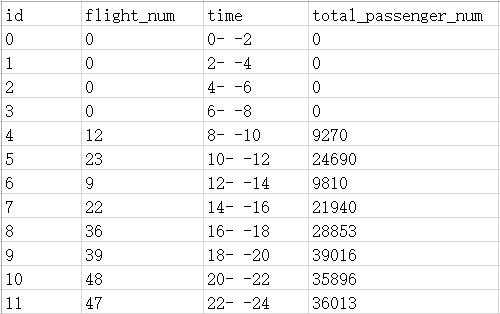
\includegraphics[width=0.7\textwidth]{figures/Data_31.png}
\caption{the data that we collected}
\label{fig:label}
\end{figure}
(The third column is the time period, the second column is the number of flights in the time period, and the fourth column is the total number of passengers in the time period)\\
For the number of people on each flight, P will choose a taxi. We check the airport traffic every 2 hours, and then based on the big data of Pudong Airport - during the day, about 15% of passengers will choose a taxi, 1.5 per car. people. In the evening, about 45% of passengers will choose a taxi, 1.5 people per car. You get the number of taxis you need every two hours, and assuming you have the same number of taxis on each flight, you can get as many taxis as you need for each flight.
Assuming that the number of taxi passengers selected on each flight is the same, you can get the number of taxis P that will be required for each flight, and the direct time interval $\Delta t$.

\begin{figure}[H]
\centering
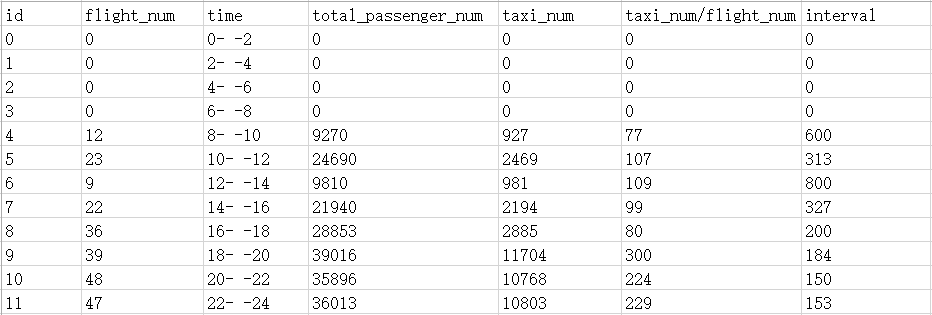
\includegraphics[width=0.7\textwidth]{figures/data3_2.png}
\caption{Flight schedule}
\label{fig:label}
\end{figure}

\item \textbf{Model calculation}\\
The initial length of the team is 0, and the airport traffic is small in the morning.
considering:
\begin{equation}\begin{split} T_{s} = \frac{{(d+k*\Delta d)}*{(n-1)}*{x}}{2}+\frac{{(d+k*\Delta d)}*{(m-1)}*{(p-x)}}{2}+t_t*(P-x)\\+\frac{{(d+k*\Delta d)}*{(n-1)}*x}{v*k}+\frac{{(d+k*\Delta d)}*{(n-1)}*(p-x)}{v*k}+\frac{c}{2}*\frac{x}{n}*\frac{x}{n*k}\\+\frac{c}{2}*\frac{P-x}{m}*+\frac{P-x}{m*k}\end{split}\end{equation}

Where d is the minimum distance of the boarding point, considering that the boarding point is relatively crowded, the taxi speed limit is 20km/h, the safety distance is 10m, take d=10, $\Delta$ d=4. There are k vehicles in the same train at the time of each batch of vehicles. Considering safety and order, they should be as small as possible. $T_t$ is the time of crossing the bridge, which is roughly set to 30s. The average speed of the taxi is considered to be 5m/s and the baggage time is 20s.
In order to find the loading point n, m and the passenger arrangement x and the taxi arrangement k which minimize the waiting time of $T_s$, the genetic algorithm is used to solve the problem. When the termination condition is reached for a certain flight, the passengers of the previous flight are still found. queue.
Substituting into the model calculation, the results are as follows. (The first column: the first flight on that day, the second column: the average number of taxis required for passengers on each flight, the third column: flight interval (seconds), the fourth column: the number of points on the L side ( n), the fifth column: the number of boarding points on the R side (m), the sixth column: the number of passengers who need to cross the bridge account for all passengers (x/p), the seventh column: the same boarding point in a group of taxis Number of cars (k), eighth column: number of queues at the pick-up point when the flight arrives (B), ninth column: model maximum number of passengers per second ($E_m$)

\begin{figure}[H]
\centering
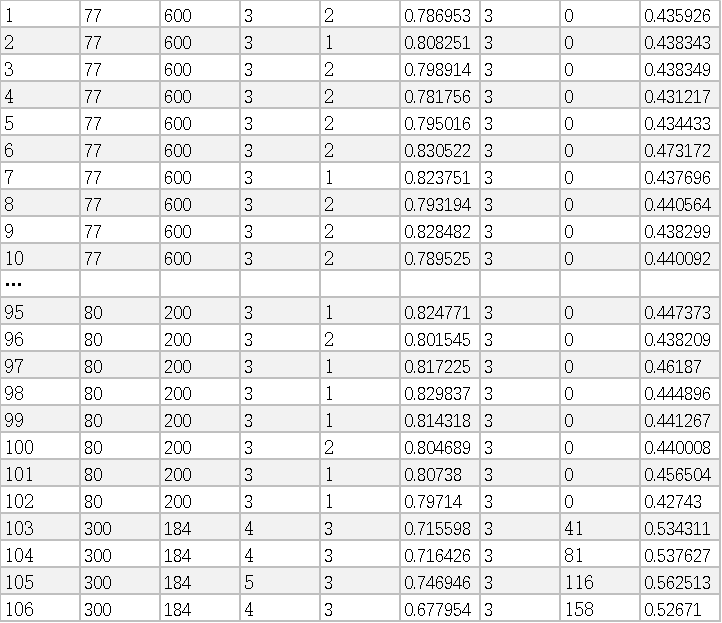
\includegraphics[width=0.7\textwidth]{figures/data3_3.png}
\caption{Calculation result table 1}
\label{fig:label}
\end{figure}

It was found that until 103 flights arrived at 6 pm, when the current flight arrived, the person on the pick-up point was waiting in line. That is, before 6 pm, all the time when the current flight arrived, it was found that there was no queue at the pick-up point. In order to minimize the total waiting time $T_s$ of all passengers, the boarding point should be arranged with 3 on the L side, 2 on the R side, and the distance between the boarding points is 18m; the vehicle arrangement is k=3, that is, each batch is rented. There are 3 consecutive vehicles to the same boarding point; passengers arrange about 1/5 passengers to pass the bridge, go to the R side to wait for the car, and let the top two of the team get on the train at the same time.
After 6 pm, the traffic volume continues to increase and reaches the peak at 22-24, using the model at this time.
\begin{equation} T_{s} = \frac{{(d+k*\Delta d)}*{(n-1)}*{(B*2*n'+p)}}{v*k}+c*\frac{2*B*n'+p}*{4*n}*{(2*B*n'+p)}\end{equation}
\begin{equation} B =B'+\frac{p}{2*n}-\frac{\Delta t*E_m}{2*n} \end{equation}
\begin{equation} v =v_1 * In[\frac{k_j}{k}]\end{equation}
The minimum distance between the vehicles on the d, considering that the boarding point is relatively crowded, the taxi speed limit is 20km / h, the safety distance is 10m, take d = 10, $\Delta$ d = 4. There are k vehicles in the same train at the time of each batch of vehicles. Considering safety and order, they should be as small as possible. The taxi speed $v_1$ considers the speed limit to be 5m/s, $k_j$ is 1/3, k=k/(10+4*k), because the passenger flow is huge at this time, so the waiter is added to serve the passengers, carry the luggage and sit on the seat. The time c is shortened to 5s.
In order to find the boarding point arrangement n and the taxi arrangement k which minimize $T_s$, that is, the waiting time, a genetic algorithm is used for solving.
Substitute the model calculation and get. (The first column: the first flight on that day, the second column: the average number of taxis required for passengers on each flight, the third column: flight interval (seconds), the fourth column: the number of passengers on one side (n ), the fifth column: the number of cars in the same boarding point in a batch of taxis (k), the sixth column: the number of people queued at the arrival point when the flight arrives (B), the seventh column: the maximum number of passengers per second in the model ( $E_m$))
\begin{figure}[H]
\centering
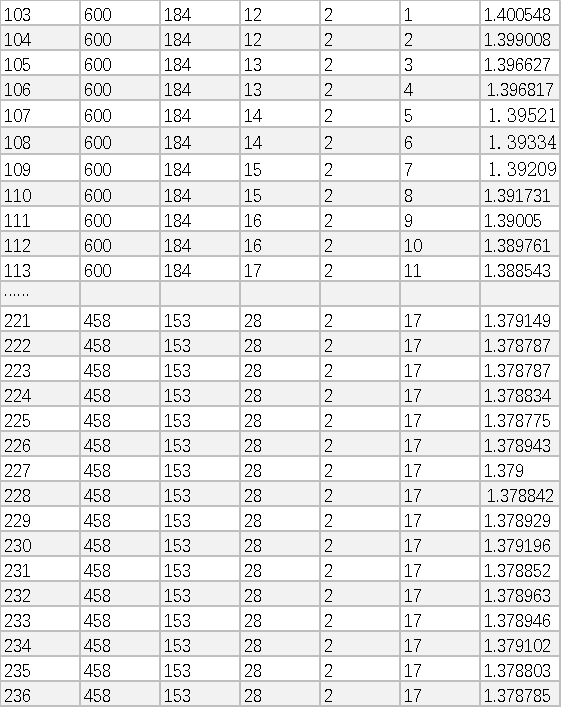
\includegraphics[width=0.7\textwidth]{figures/data3_4.png}
\caption{Calculation result table 2}
\label{fig:label}
\end{figure}
It can be seen that after 6 pm, 28 parking spots need to be arranged on the side of the road. The distance between each parking point is 122 meters. If this arrangement is arranged, the waiting team will not increase any more when it is increased to a certain length. The length is 17, because the total number is 17*33*2, and the maximum number of passengers per second is 1.358. Therefore, the last passenger can take about 15 minutes to wait until the car, and the model service capability is acceptable.
By sorting the number of points printed on the above into a picture, you can see the number of boarding points that should be arranged for each time period.
\begin{figure}[H]
\centering
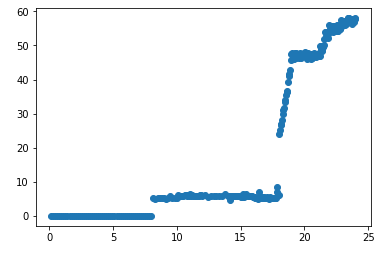
\includegraphics[width=0.7\textwidth]{figures/data3_5.png}
\caption{Boarding time period chart}
\label{fig:label}
\end{figure}
0 to 8 o'clock, the total number of boarding points is 0;
From 8:00 to 18:00, the total number of boarding points is 5, 3 on one side and 2 on the other side;
From 18 o'clock to 22:00, the total number of boarding points is 46, 23 on one side and 23 on the other side;
From 22 o'clock to 24:00, the total number of boarding points is 56, 28 on one side and 28 on the other.

\item \textbf{Model rationality analysis}\\
We found information about Pudong International Airport:\\
1. Passengers can get on the bus within an average of 20 minutes during peak hours, which is basically consistent with the model;\\
2. Pudong Airport arranged a “baggage ambassador” in uniform to help when the passenger flow was large, which was consistent with the model assumptions;\\
3. Pudong Airport will issue a card to the taxi driver to specify the driver's pick-up point to be driven, which is consistent with our model assumptions;\\
4. Pudong Airport arranged a corresponding pick-up point for each taxi, which is consistent with the model assumptions. Pudong International Airport has a maximum of 12 pick-up points, and we have calculated 56. The difference is so great. The reasons we analyzed are: the road at the pick-up point of Pudong International Airport can accommodate more than two vehicles, and the pick-up point Can be scattered in all directions of the airport; and the problem requires that the boarding point road can only accommodate two cars, and all the loading points are concentrated on one road, so our model has less space in the scheduling, in order to meet the same The magnitude of the passenger flow leads to deviations in the results.

\end{enumerate}



